\subsection{Comparison Charts} \label{section:appendix:charts}

\textbf{NOTE:} The following charts are a summary of the data collected from the performance tests executed, which can be found in the project's repository. Each test was performed five times, being also run an extra time for C++ line and block multiplications to gather L3 cache misses data. The median was used in the chart generation to represent the data for each value set.

    \begin{figure}[ht]
        \centering
        \captionsetup{justification=centering, margin=2cm}
        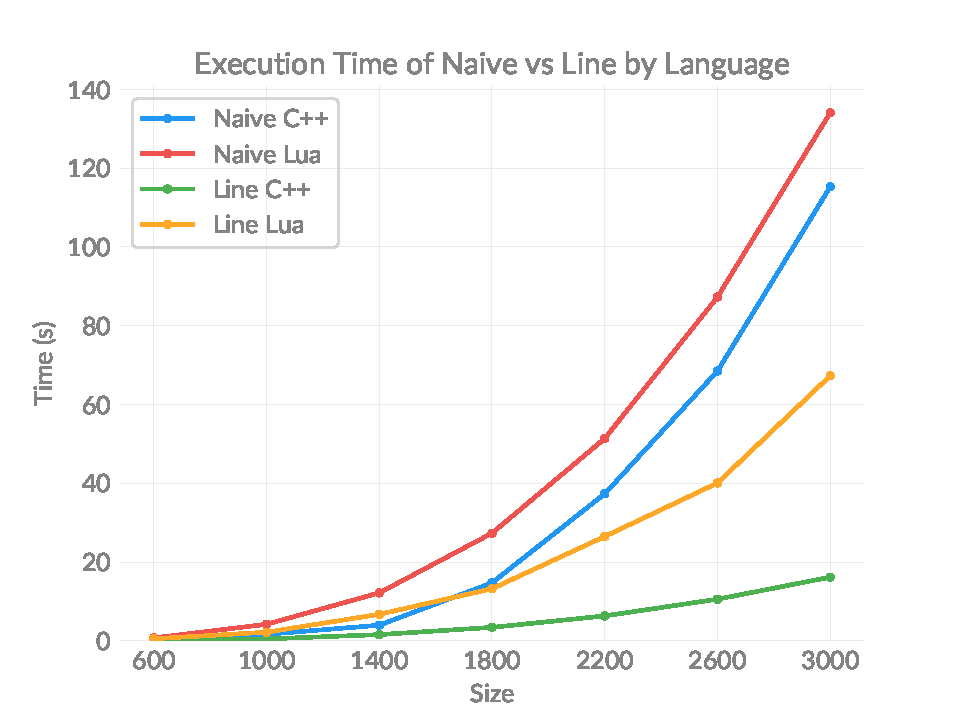
\includegraphics[width=0.8\textwidth]{pdf/naive-line-time}
        \caption{Time comparison between naive and line multiplication, in both C++ and Lua}
        \label{fig:chart:naive-line-time}
    \end{figure}

    \begin{figure}[ht]
        \centering
        \captionsetup{justification=centering, margin=2cm}
        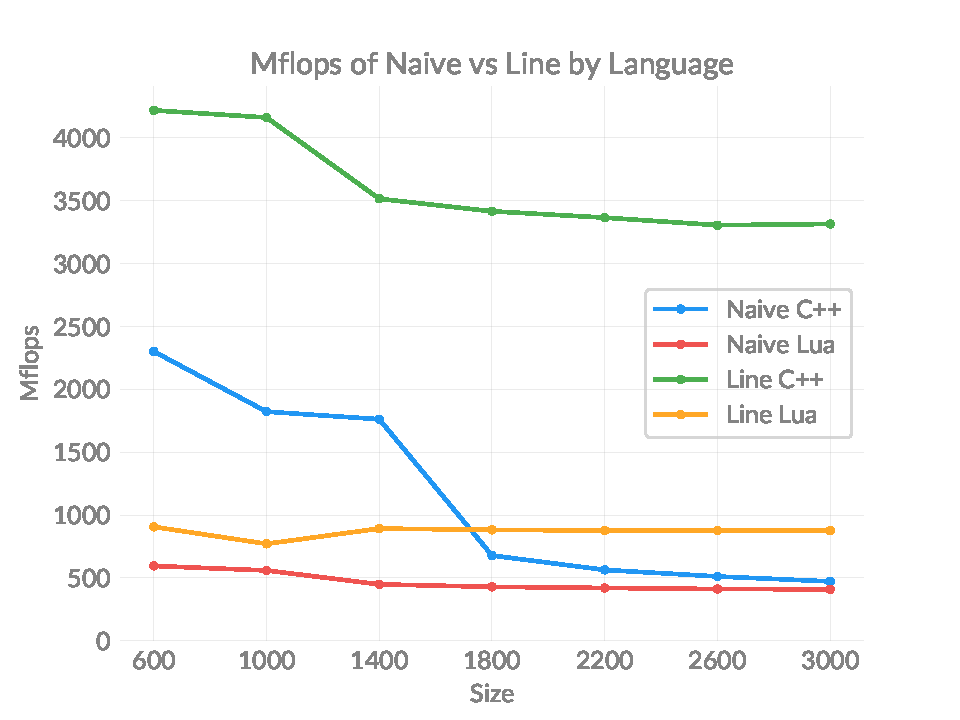
\includegraphics[width=0.8\textwidth]{pdf/naive-line-flops}
        \caption{Mflops comparison between naive and line multiplication, in both C++ and Lua}
        \label{fig:chart:naive-line-flops}
    \end{figure}

    \begin{figure}[ht]
        \centering
        \captionsetup{justification=centering, margin=2cm}
        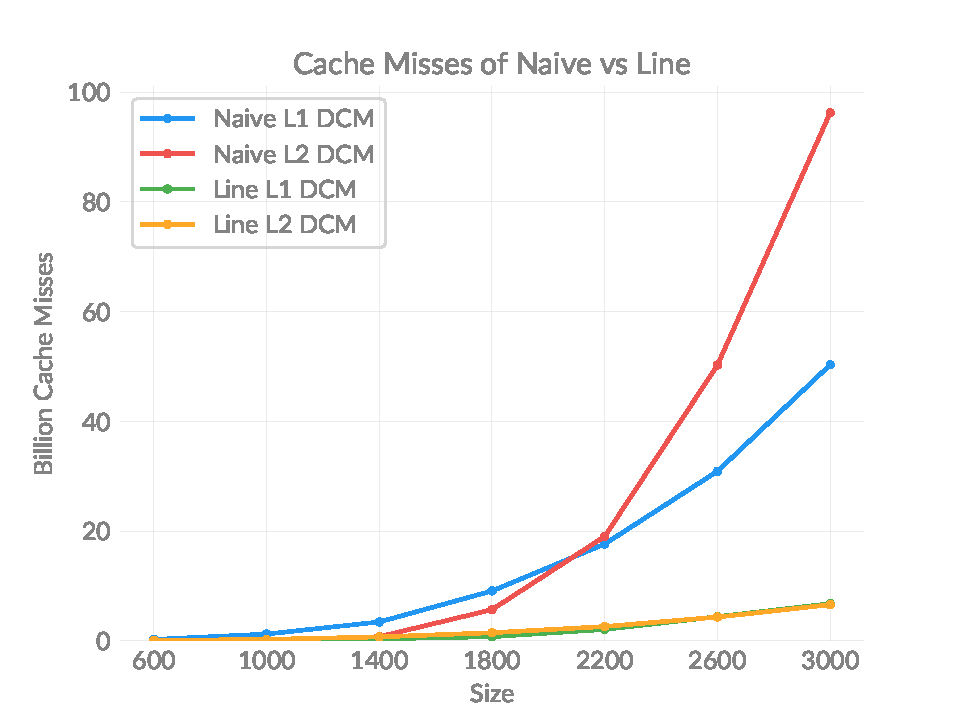
\includegraphics[width=0.8\textwidth]{pdf/naive-line-cache}
        \caption{Cache misses comparison between naive and line multiplication, in C++}
        \label{fig:chart:naive-line-cache}
    \end{figure}

    \begin{figure}[ht]
        \centering
        \captionsetup{justification=centering, margin=2cm}
        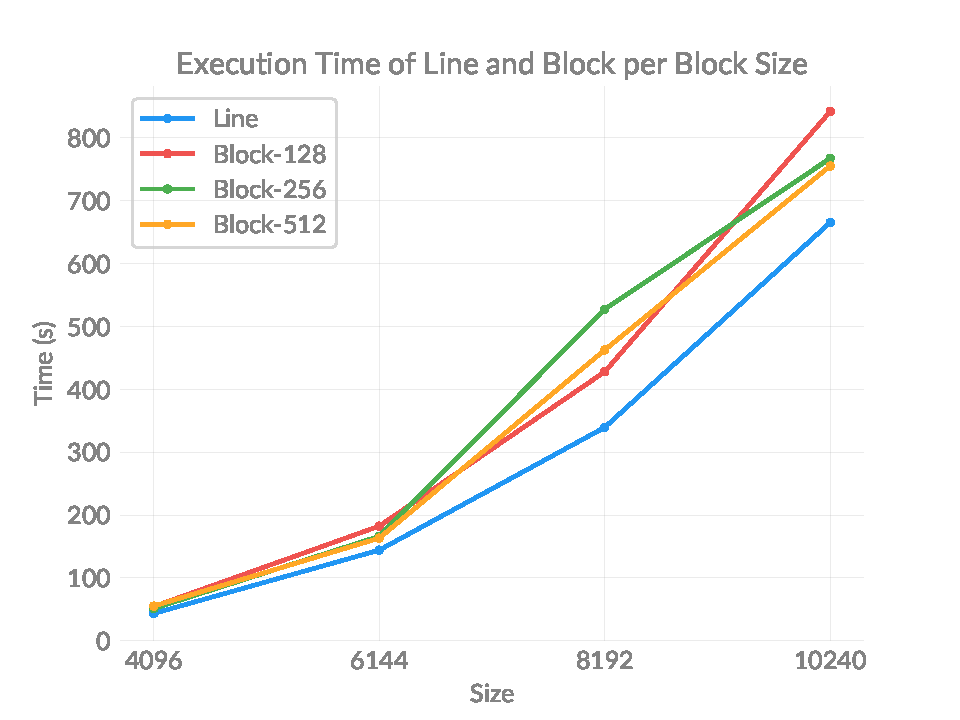
\includegraphics[width=0.8\textwidth]{pdf/line-block-time}
        \caption{Time comparison between line and block multiplication, with different block sizes}
        \label{fig:chart:line-block-time}
    \end{figure}

    \begin{figure}[ht]
        \centering
        \captionsetup{justification=centering, margin=2cm}
        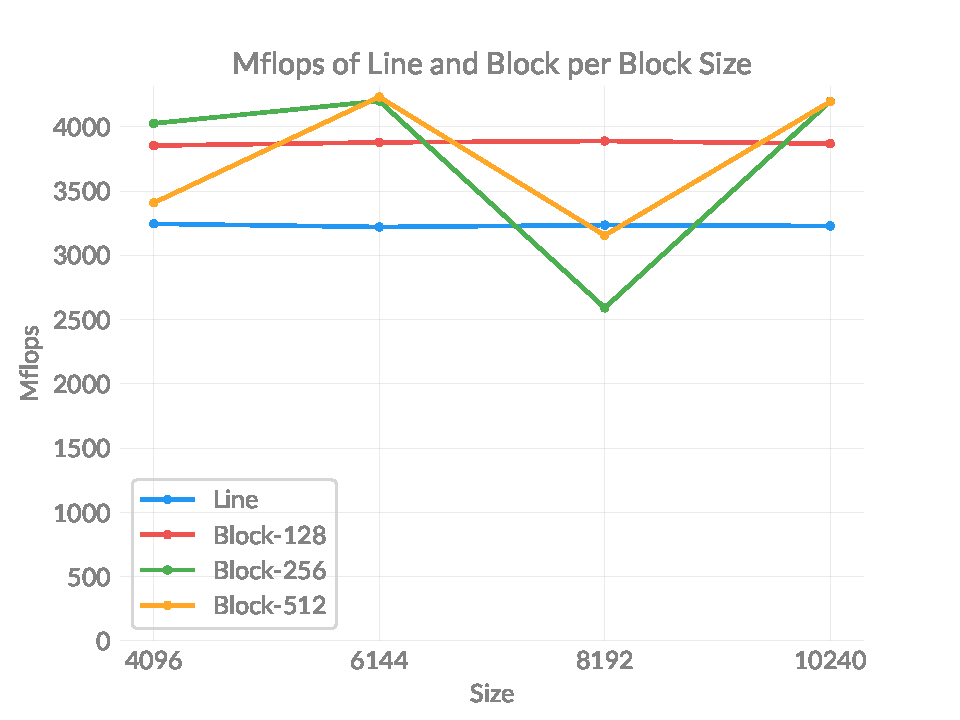
\includegraphics[width=0.8\textwidth]{pdf/line-block-flops}
        \caption{Mflops comparison between line and block multiplication, with different block sizes}
        \label{fig:chart:line-block-flops}
    \end{figure}

    \begin{figure}[ht]
        \centering
        \captionsetup{justification=centering, margin=2cm}
        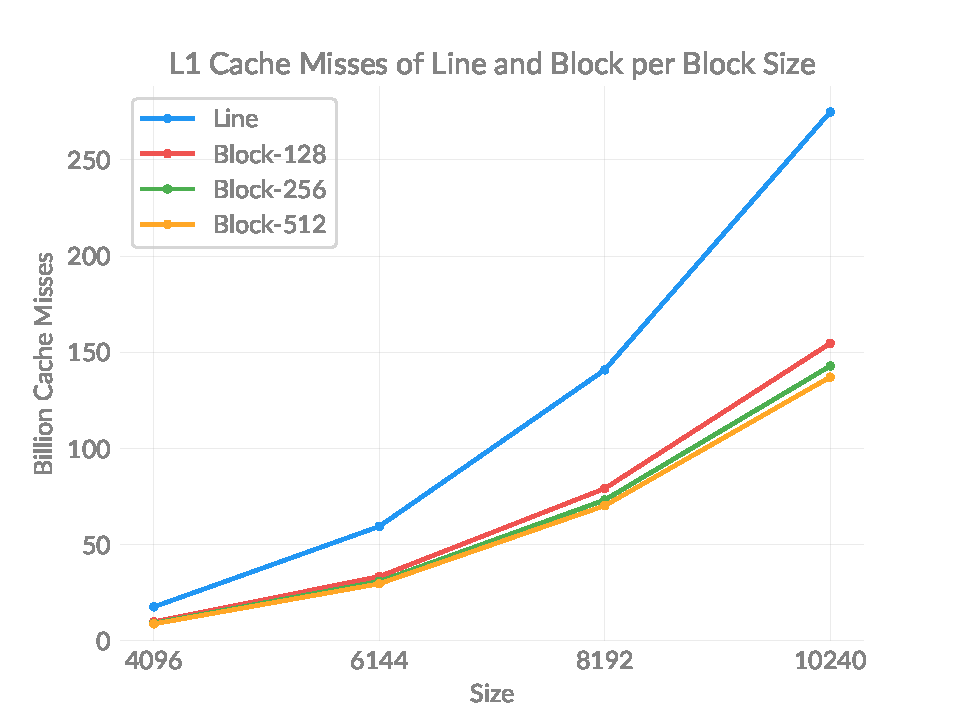
\includegraphics[width=0.8\textwidth]{pdf/line-block-l1}
        \caption{L1 cache miss comparison between line and block multiplication, with different block sizes}
        \label{fig:chart:line-block-l1}
    \end{figure}

    \begin{figure}[ht]
        \centering
        \captionsetup{justification=centering, margin=2cm}
        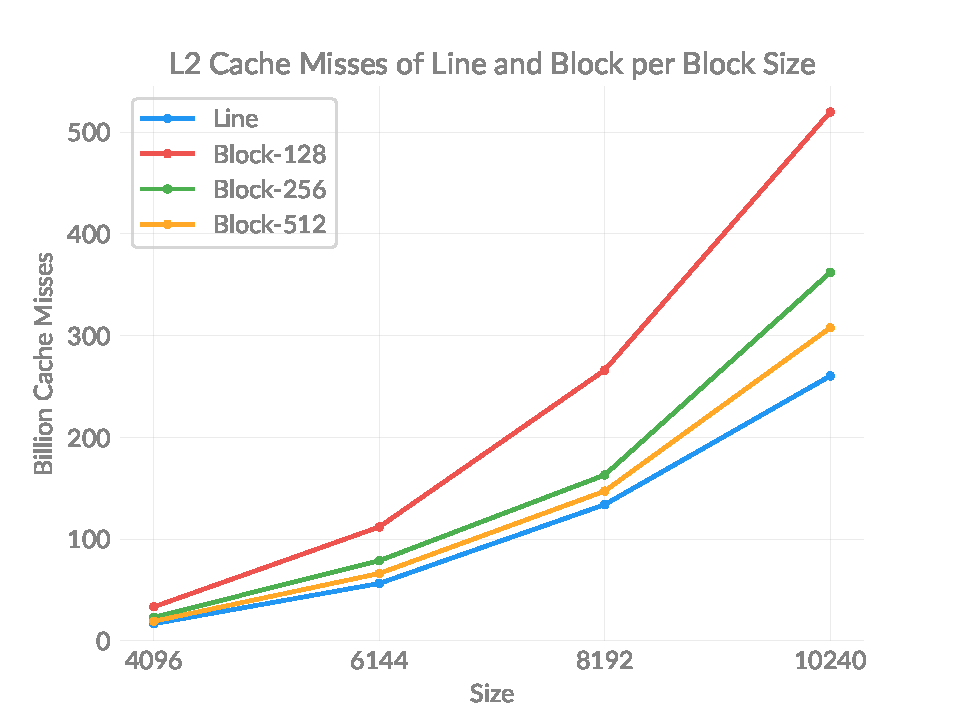
\includegraphics[width=0.8\textwidth]{pdf/line-block-l2}
        \caption{L2 cache miss comparison between line and block multiplication, with different block sizes}
        \label{fig:chart:line-block-l2}
    \end{figure}

    \begin{figure}[ht]
        \centering
        \captionsetup{justification=centering, margin=2cm}
        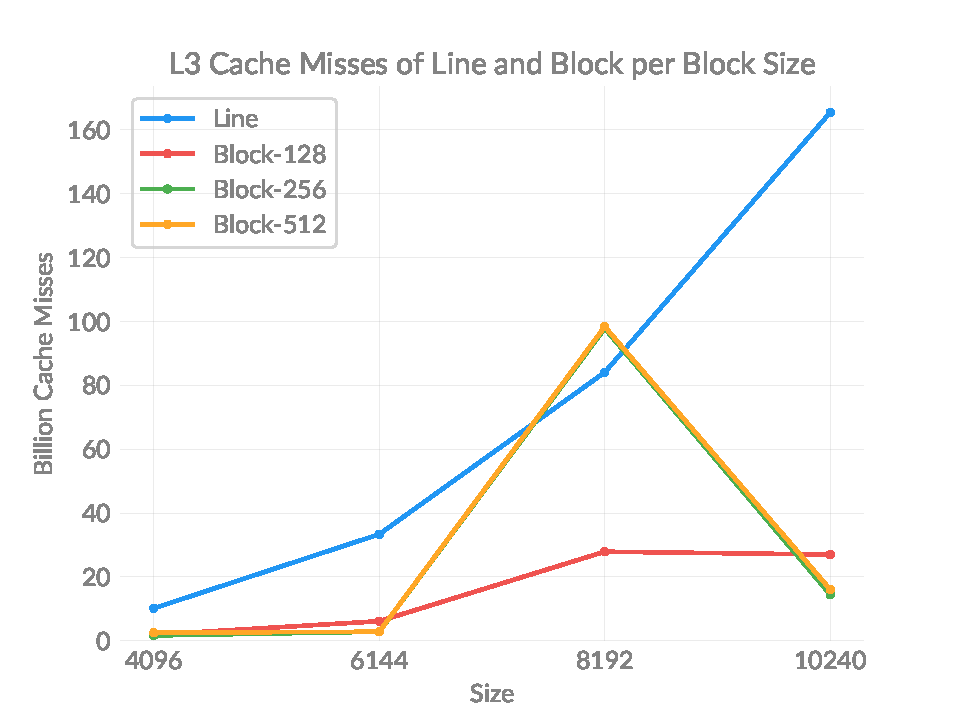
\includegraphics[width=0.8\textwidth]{pdf/line-block-l3}
        \caption{L3 cache miss comparison between line and block multiplication, with different block sizes}
        \label{fig:chart:line-block-l3}
    \end{figure}

    \begin{figure}[ht]
        \centering
        \captionsetup{justification=centering, margin=2cm}
        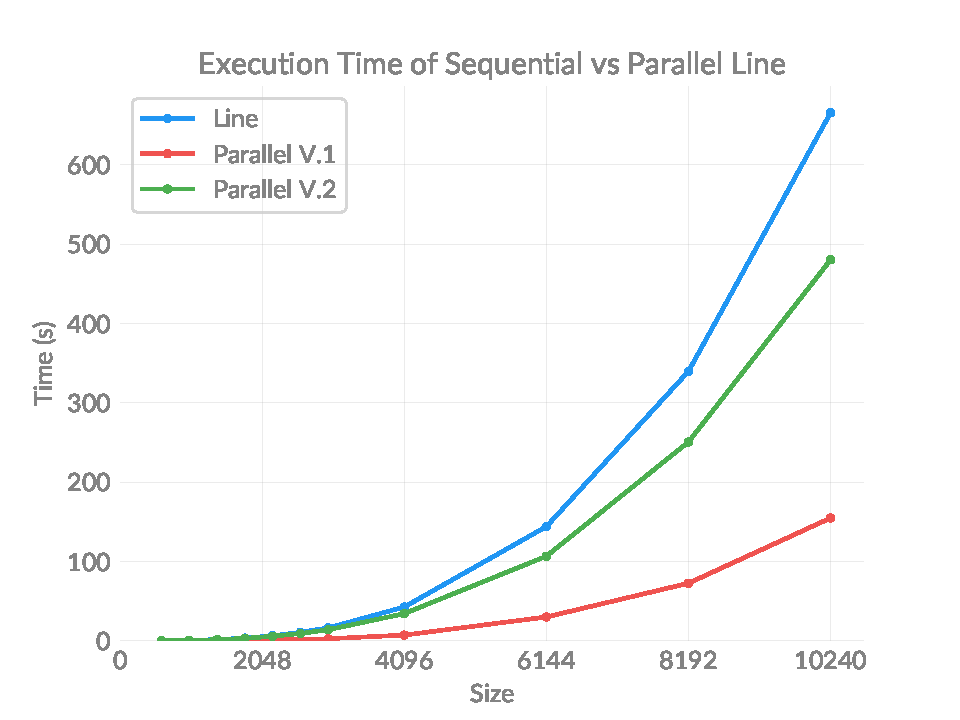
\includegraphics[width=0.8\textwidth]{pdf/parallel-time}
        \caption{Time comparison between sequential and parallel line multiplication}
        \label{fig:chart:parallel-time}
    \end{figure}

    \begin{figure}[ht]
        \centering
        \captionsetup{justification=centering, margin=2cm}
        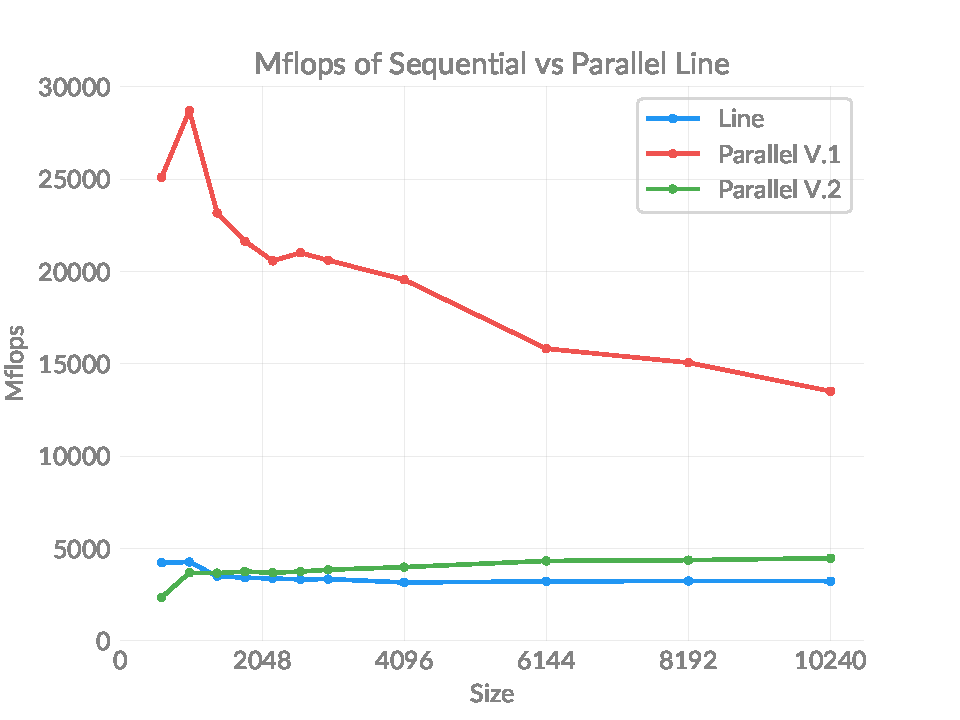
\includegraphics[width=0.8\textwidth]{pdf/parallel-flops}
        \caption{Mflops comparison between sequential and parallel line multiplication}
        \label{fig:chart:parallel-flops}
    \end{figure}

    \begin{figure}[ht]
        \centering
        \captionsetup{justification=centering, margin=1.2cm}
        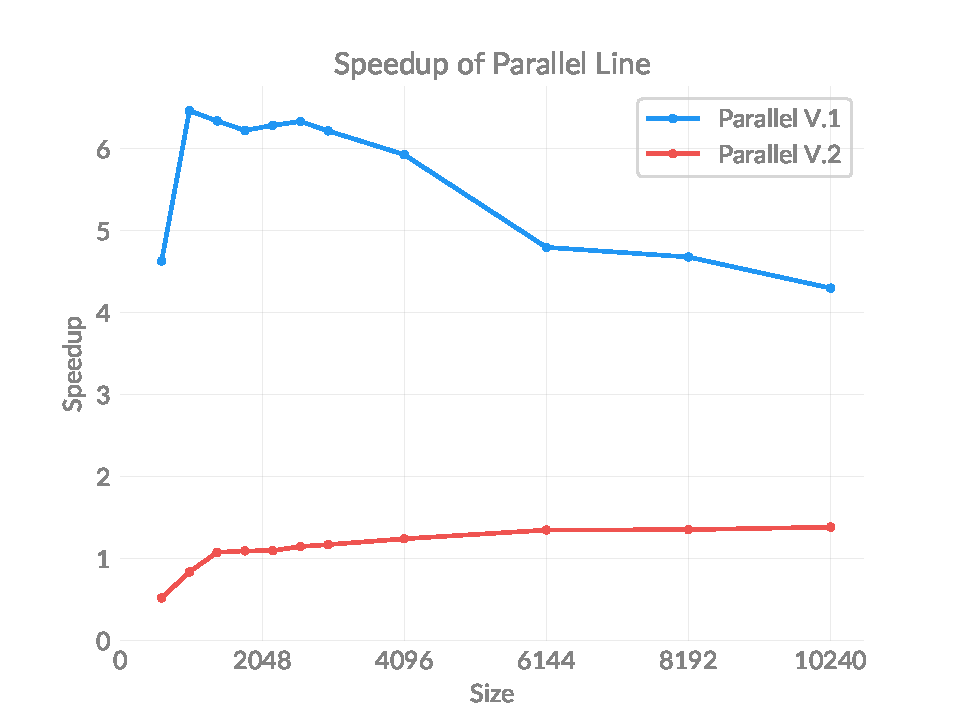
\includegraphics[width=0.8\textwidth]{pdf/parallel-speedup}
        \caption{Speedup comparison between versions of parallel line multiplication, relative to the sequential version}
        \label{fig:chart:parallel-speedup}
    \end{figure}

    \begin{figure}[ht]
        \centering
        \captionsetup{justification=centering, margin=1.2cm}
        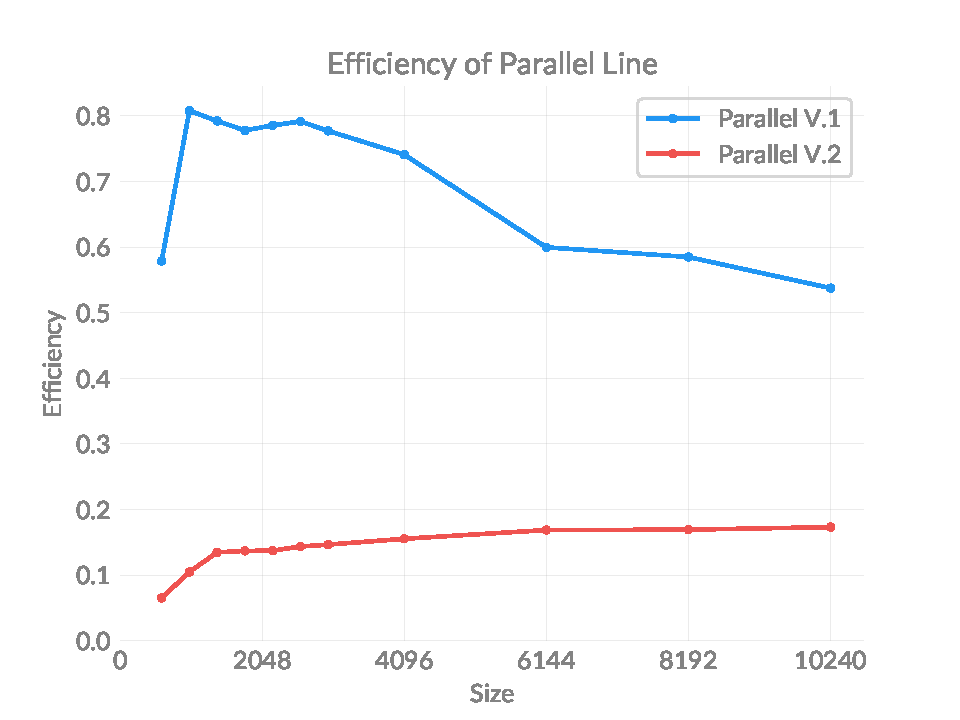
\includegraphics[width=0.8\textwidth]{pdf/parallel-efficiency}
        \caption{Efficiency comparison between versions of parallel line multiplication, relative to the sequential version}
        \label{fig:chart:parallel-efficiency}
    \end{figure}

\clearpage